
\begin{correction} \;
\begin{enumerate}
\item \textbf{\'Etudier les variations de la fonction $f: x\mapsto \ddp\frac{3}{4}x^2-2x+3$ associ\'ee:}
\begin{itemize}
\item[$\bullet$] La fonction $f$ est bien d\'efinie sur $\R$ comme fonction polynomiale.
\item[$\bullet$] La fonction $f$ est d\'erivable sur $\R$ comme fonction polynomiale et pour tout $x\in\R$: 
$f^{\prime}(x)=\ddp\frac{3}{2}x-2$.
\item[$\bullet$] On obtient ainsi les variations suivantes:
\begin{center}
\begin{tikzpicture}
 \tkzTabInit{ $x$          /1,%
       $f'(x)$      /1,%
       $f$       /2}%
     { $-\infty$, $\ddp\frac{4}{3}$ ,$+\infty$ }%
  \tkzTabLine {,-,0,+,}%
  \tkzTabVar{
       +/ $+\infty$        /,
        -/$\ddp\frac{5}{3}$           /,%
       +/$+\infty$           /,
                      }
 \tkzTabVal[draw]{2}{3}{0.3}{$2$}{$2$}
\end{tikzpicture}
\end{center}
\item[$\bullet$] Les limites en $\pm\infty$ s'obtiennent avec le th\'eor\`{e}me du mon\^{o}me de plus haut degr\'e.
\end{itemize}
\item \textbf{\'Etudier le signe de la fonction $g: x\mapsto f(x)-x=\ddp\frac{3}{4}x^2-3x+3$:}\\
\noindent Le discriminant vaut $\Delta=0$ et l'unique racine est 2. Ainsi

 \fbox{la fonction $g$ est positive sur $\R$ et ne s'annule qu'en 2.}
\item \textbf{Calculer les limites \'eventuelles de la suite $\suiteu$:}\\
\noindent On suppose que la suite $\suiteu$ converge vers un r\'eel $l\in\mathcal{D}_f=\R$.
\begin{itemize}
\item[$\star$] On a donc:
\begin{itemize}
\item[$\circ$] La suite converge vers $l$.
\item[$\circ$] La fonction $f$ est continue sur $\R$ comme fonction polynomiale donc elle est en particulier continue en $l$.
\end{itemize}
Donc d'apr\`{e}s le th\'eor\`{e}me sur les suite et fonction, on obtient que: $\lim\limits_{n\to +\infty} f(u_n)=f(l)$.
\item[$\star$] De plus on a: $\lim\limits_{n\to +\infty} u_{n+1}=l$.
\item[$\star$] On peut donc passer \`{a} la limite dans l'\'egalit\'e: $u_{n+1}=f(u_n)$ et on obtient que: $l=f(l)$/
\item[$\star$] On a donc: $l=f(l)\Leftrightarrow g(l)=0\Leftrightarrow l=2$. \\
\noindent \fbox{La seule limite \'eventuelle est 2.}
\end{itemize}
\item \textbf{On suppose que $u_0>2$:}
\begin{enumerate}
\item \textbf{Montrer que la suite est bien d\'efinie et que pour tout $n\in\N$: $u_n>2$:}\\
\noindent On peut commencer par montrer que l'intervalle $\rbrack 2,+\infty\lbrack$ est stable par $f$. 
%On a:
%\begin{itemize}
%\item[$\circ$] La fonction $f$ est continue sur $\rbrack 2,+\infty\lbrack$.
%\item[$\circ$] La fonction $f$ est strictement croissante sur $\rbrack 2,+\infty\lbrack$.
%\item[$\circ$] $f(2)=2$ et $\lim\limits_{x\to +\infty} f(x)=+\infty$.
%\end{itemize}
%Ainsi d'apr\`{e}s le th\'eor\`{e}me de la bijection, on a en particulier que $f(\rbrack 2,+\infty\lbrack)=\rbrack 2,+\infty\lbrack$. Et comme $\rbrack 2,+\infty\lbrack \subset \rbrack 2,+\infty\lbrack$, \fbox{l'intervalle $\rbrack 2,+\infty\lbrack$ est stable par $f$.} 
On a $f$ strictement croissante sur $[2,+\infty[$, et $f(2) =2$. Donc pour tout $x \in [2,+\infty[, f(x) > 2$ et l'intervalle  $\rbrack 2,+\infty\lbrack$ est stable par $f$.\\
On montre par r\'ecurrence sur $n\in\N$ la propri\'et\'e : $\mathcal{P}(n):\ u_n\ \hbox{existe et}\ u_n>2.$
\begin{itemize}
\item[$\star$] Initialisation: pour $n=0$: par d\'efinition de la suite, $u_0$ existe et $u_0>2$. Donc $\mathcal{P}(0)$ est vraie.
\item[$\star$] H\'er\'edit\'e: soit $n\in\N$ fix\'e, on suppose que la propri\'et\'e vraie \`{a} l'ordre $n$, montrons que $\mathcal{P}(n+1)$ est vraie. Par hypoth\`{e}se de r\'ecurrence, on sait que $u_n$ existe et que $u_n>2$. Donc $f(u_n)$ existe c'est-\`{a}-dire $u_{n+1}$ existe. De plus, l'intervalle $\rbrack 2,+\infty\lbrack$ est stable par $f$. Donc $f(u_n)>2$ c'est-\`{a}-dire $u_{n+1}>2$.
Donc $\mathcal{P}(n+1)$ est vraie.
\item[$\star$] Conclusion: il r\'esulte du principe de r\'ecurrence que

 \fbox{la suite $\suiteu$ est bien d\'efinie et que pour tout $n\in\N,\ u_n>2.$}
\end{itemize}
\item \textbf{\'Etudier la monotonie de la suite $\suiteu$:}\\
\noindent Soit $n\in\N$, on a: $u_{n+1}-u_n=f(u_n)-u_n=g(u_n)$. Ainsi comme le signe de $g$ est positif sur $\R$, on obtient que pour tout $n\in\N$: $u_{n+1}-u_n\geq 0$. Ainsi \fbox{la suite $\suiteu$ est croissante.}
\item \textbf{\'Etudier le comportement \`{a} l'infini de la suite $\suiteu$:}
\begin{itemize}
\item[$\star$] La suite $\suiteu$ est croissante donc d'apr\`{e}s le th\'eor\`{e}me sur les suites monotones, elle converge ou elle diverge vers $+\infty$.
\item[$\star$] On suppose par l'absurde que la suite $\suiteu$ converge vers un r\'eel $l$. On a alors:
\begin{itemize}
\item[$\circ$] La suite $\suiteu$ converge vers $l$.
\item[$\circ$] Comme la suite $\suiteu$ est croissante, on a pour tout $n\in\N$: $u_n\geq u_0$.
\end{itemize}
D'apr\`{e}s le th\'eor\`{e}me de passage \`{a} la limite, on obtient donc que: $l\geq u_0$. Or par hypoth\`{e}se, on sait que $u_0>2$. Ainsi on obtient que: $l>2$. Absurde car la seule limite \'eventuelle de la suite $\suiteu$ est 2. Ainsi \fbox{la suite $\suiteu$ diverge vers $+\infty$.}
\end{itemize}
\end{enumerate}
\item \textbf{On suppose que $u_0\in\left\rbrack \ddp\frac{2}{3},2\right\lbrack $:}
\begin{enumerate}
\item \textbf{Montrer que la suite est bien d\'efinie et que pour tout $n\in\N$: $u_n\left\rbrack \ddp\frac{2}{3},2\right\lbrack$:}\\
\noindent On peut commencer par montrer que l'intervalle $\left\rbrack \ddp\frac{2}{3},2\right\lbrack$ est stable par $f$. Attention, ici $f$ n'est pas monotone sur $\left\rbrack \ddp\frac{2}{3},2\right\lbrack$, il faut donc traiter les deux intervalles $\left\rbrack \ddp\frac{2}{3},\ddp\frac{4}{3}\right\rbrack$ et $\left\rbrack \ddp\frac{4}{3}, 2\right\rbrack$ s\'eparemment.\\
Sur $\left\rbrack \ddp\frac{2}{3},\ddp\frac{4}{3}\right\rbrack$, $f$ est strictement d\'ecroissante et $f\left(\ddp\frac{2}{3}\right) = 2$, $f\left(\ddp\frac{4}{3}\right)=\ddp\frac{5}{3}$. Donc pour tout $x \in \left\rbrack \ddp\frac{2}{3},\ddp\frac{4}{3}\right\rbrack$, $f(x) \in \left\rbrack \ddp\frac{5}{3},2\right\rbrack$, donc $f(x) \in \left\rbrack \ddp\frac{2}{3},2\right\lbrack$.\\
Sur $\left\rbrack\ddp\frac{4}{3},2\right\rbrack$, $f$ est strictement croissante et $f\left(2\right) = 2$, $f\left(\ddp\frac{4}{3}\right)=\ddp\frac{5}{3}$. Donc pour tout $x \in \left\rbrack \ddp\frac{4}{3},2\right\rbrack$, $f(x) \in \left\rbrack \ddp\frac{5}{3},2\right\rbrack$, donc $f(x) \in \left\rbrack \ddp\frac{2}{3},2\right\lbrack$.\\
En en d\'eduit que pour tout $x \in \left\rbrack \ddp\frac{2}{3},2\right\lbrack$, on a bien $f(x) \in \left\rbrack \ddp\frac{2}{3},2\right\lbrack$ : l'intervalle $\left\rbrack \ddp\frac{2}{3},2\right\lbrack$ est stable par $f$.\\
%On a:
%\begin{itemize}
%\item[$\circ$] La fonction $f$ est continue sur $\left\rbrack \ddp\frac{2}{3},\ddp\frac{4}{3}\right\rbrack$.
%\item[$\circ$] La fonction $f$ est strictement d\'ecroissante sur $\left\rbrack \ddp\frac{2}{3},\ddp\frac{4}{3}\right\rbrack$.
%\item[$\circ$] $f\left( \ddp\frac{2}{3}\right)=2$ et $f\left( \ddp\frac{4}{3}\right)=\ddp\frac{5}{3}$.
%\end{itemize}
%Ainsi d'apr\`{e}s le th\'eor\`{e}me de la bijection, on a en particulier que $f(\left\rbrack \ddp\frac{2}{3},\ddp\frac{4}{3}\right\rbrack)=\left\lbrack \ddp\frac{5}{3},2\right\lbrack$. \\
%\noindent On a aussi:
%\begin{itemize}
%\item[$\circ$] La fonction $f$ est continue sur $\left\lbrack \ddp\frac{4}{3},2\right\lbrack$.
%\item[$\circ$] La fonction $f$ est strictement croissante sur $\left\lbrack \ddp\frac{4}{3},2\right\lbrack$.
%\item[$\circ$] $f\left(2\right)=2$ et $f\left( \ddp\frac{4}{3}\right)=\ddp\frac{5}{3}$.
%\end{itemize}
%Ainsi d'apr\`{e}s le th\'eor\`{e}me de la bijection, on a en particulier que $f(\left\lbrack \ddp\frac{4}{3},2\right\lbrack)=\left\lbrack \ddp\frac{5}{3},2\right\lbrack$. \\
%\noindent Au final on obtient donc que: 
%$$f(\left\rbrack \ddp\frac{2}{3},2\right\lbrack)=f(\left\rbrack \ddp\frac{2}{3},\ddp\frac{4}{3}\right\rbrack)\cup f(\left\lbrack \ddp\frac{4}{3},2\right\lbrack)=\left\lbrack \ddp\frac{5}{3},2\right\lbrack\cup\left\lbrack \ddp\frac{5}{3},2\right\lbrack=\left\lbrack \ddp\frac{5}{3},2\right\lbrack.$$
%Et comme $\left\lbrack \ddp\frac{5}{3},2\right\lbrack \subset \left\rbrack \ddp\frac{2}{3},2\right\lbrack$, \fbox{l'intervalle $\left\rbrack \ddp\frac{2}{3},2\right\lbrack$ est stable par $f$.} 
On montre par r\'ecurrence sur $n\in\N$ la propri\'et\'e $\mathcal{P}(n):\ u_n\ \hbox{existe et}\ u_n\in\left\rbrack \ddp\frac{2}{3},2\right\lbrack.$
\begin{itemize}
\item[$\star$] Initialisation: pour $n=0$: par d\'efinition de la suite, $u_0$ existe et $u_0\in\left\rbrack \ddp\frac{2}{3},2\right\lbrack$. Donc $\mathcal{P}(0)$ est vraie.
\item[$\star$] H\'er\'edit\'e: soit $n\in\N$ fix\'e, on suppose que la propri\'et\'e vraie \`{a} l'ordre $n$, montrons que $\mathcal{P}(n+1)$ est vraie.
Par hypoth\`{e}se de r\'ecurrence, on sait que $u_n$ existe et que $u_n\in\left\rbrack \ddp\frac{2}{3},2\right\lbrack$. Donc $f(u_n)$ existe c'est-\`{a}-dire $u_{n+1}$ existe.\\
De plus, $u_n\in\left\rbrack \ddp\frac{2}{3},2\right\lbrack$. Or l'intervalle $\left\rbrack \ddp\frac{2}{3},2\right\lbrack$ est stable par $f$. Donc $f(u_n)\in\left\rbrack \ddp\frac{2}{3},2\right\lbrack$ c'est-\`{a}-dire $u_{n+1}\in\left\rbrack \ddp\frac{2}{3},2\right\lbrack$. Donc $\mathcal{P}(n+1)$ est vraie.
\item[$\star$] Conclusion: il r\'esulte du principe de r\'ecurrence que

 \fbox{la suite $\suiteu$ est bien d\'efinie et que pour tout $n\in\N,\ u_n\in\left\rbrack \ddp\frac{2}{3},2\right\lbrack.$}
\end{itemize}
\item \textbf{\'Etudier la monotonie de la suite $\suiteu$:}\\
\noindent Soit $n\in\N$, on a: $u_{n+1}-u_n=f(u_n)-u_n=g(u_n)$. Ainsi comme le signe de $g$ est positif sur $\R$, on obtient que pour tout $n\in\N$: $u_{n+1}-u_n\geq 0$. Ainsi \fbox{la suite $\suiteu$ est croissante.}
\item \textbf{\'Etudier le comportement \`{a} l'infini de la suite $\suiteu$:}
\begin{itemize}
\item[$\star$] La suite $\suiteu$ est croissante et major\'ee par 2 donc d'apr\`{e}s le th\'eor\`{e}me sur les suites monotones, elle converge.
\item[$\star$] Comme la seule limite \'eventuelle est 2, \fbox{la suite $\suiteu$ converge vers 2.}
\end{itemize}
\end{enumerate} 
\end{enumerate}
\end{correction}